% Bab II  Isi Penulisan Skripsi
\chapter{ISI PENULISAN SKRIPSI}

Penulisan skripsi merupakan bagian terpenting dari seluruh proses kegiatan penelitian yang telah dilakukan, karena dalam laporan itu semua ide dan hasil kegiatan dapat disampaikan kepada orang lain, termasuk orang yang disiplin ilmunya berbeda. Laporan harus jelas mengungkapkan semua kegiatan dan hasil-hasilnya secara sistematis, efisien dan efektif menggunakan Bahasa Indonesia yang baik dan benar.

Bab ini menguraikan isi setiap bagian skripsi: bagian awal, bagian isi (Bab I sampai Bab V), dan bagian akhir. Contoh tampilan halaman tersedia pada template Proposal, Seminar Hasil, dan Skripsi.

\section{Bagian Awal}

\subsection{Halaman Sampul}
Halaman sampul memuat, berurutan dari atas ke bawah dan seluruhnya di tengah halaman:
\begin{enumerate}
\item jenis dokumen (PROPOSAL SKRIPSI, SEMINAR HASIL, atau SKRIPSI);
\item judul penelitian, ditulis dengan huruf kapital, dicetak tebal, dan paling banyak 15 kata tanpa singkatan yang tidak lazim;
\item pernyataan maksud pengajuan, misalnya “Diajukan untuk memenuhi salah satu syarat memperoleh gelar Sarjana Komputer (S.Kom.)” (khusus skripsi);
\item logo Universitas Muhammadiyah Buton berukuran sekitar 4 sampai 5 cm;
\item “Disusun oleh”, nama lengkap mahasiswa (tanpa gelar), dan Nomor Pokok Mahasiswa (NPM);
\item PROGRAM STUDI REKAYASA SISTEM KOMPUTER, FAKULTAS TEKNIK, UNIVERSITAS MUHAMMADIYAH BUTON, kota (BAUBAU), dan tahun penyelesaian, seluruhnya huruf kapital.
\end{enumerate}
Halaman sampul dihitung sebagai halaman pertama tetapi nomornya tidak ditampilkan.

\subsection{Halaman Pengajuan dan Lembar Persetujuan Pembimbing}
Lembar ini memuat identitas mahasiswa (nama, NPM, dan kontak berupa alamat, nomor telepon, serta surel) dan persetujuan dosen pembimbing. Dosen pembimbing I dan II menandatangani lembar ini sebagai tanda bahwa dokumen layak diseminarkan atau diujikan. Nama dan NIDN dosen ditulis lengkap dengan gelar di bawah tanda tangan. Halaman ini tidak diberi nomor.

\subsection{Halaman Pengesahan}
Halaman pengesahan diberikan setelah skripsi dipertahankan di depan penguji dan telah diperbaiki sesuai masukan penguji. Halaman ini memuat judul, nama dan NPM mahasiswa, serta tanda tangan dosen pembimbing I dan II, dosen penguji, Ketua Program Studi, dan Dekan Fakultas Teknik. Tanda tangan dibubuhkan di ruang kosong di atas nama terang, tanpa kotak. Salinan yang dijilid harus memuat tanda tangan asli.

\subsection{Pernyataan Keaslian}
Pernyataan keaslian berisi pernyataan mahasiswa bahwa skripsi adalah karya sendiri, bukan hasil plagiat, dan bahwa semua sumber telah dirujuk dengan benar. Pernyataan ditulis atas nama pribadi, memuat nama, NPM, program studi, tempat dan tanggal, serta ditandatangani oleh mahasiswa.

\subsection{Abstrak}
Abstrak adalah ringkasan seluruh isi penelitian, ditulis dalam dua bahasa: Indonesia (\textit{Abstrak}) dan Inggris (\textit{Abstract}). Ketentuannya:
\begin{enumerate}
\item terdiri atas satu paragraf, \textbf{maksimal 300 kata}, ditulis dengan jarak satu spasi;
\item memuat berurutan: latar belakang singkat, tujuan, metode, hasil utama, dan kesimpulan (serta saran bila perlu);
\item tidak memuat sitasi, tabel, gambar, persamaan panjang, maupun singkatan yang belum dijelaskan;
\item diakhiri \textbf{kata kunci} (\textit{keywords}) sebanyak tiga sampai lima kata atau frasa;
\item pada proposal, abstrak menggunakan bentuk “akan” karena penelitian belum dilaksanakan.
\end{enumerate}

\subsection{Kata Pengantar}
Kata pengantar berisi ucapan syukur dan ucapan terima kasih kepada pihak yang membantu penyelesaian skripsi, disusun berurutan menurut peran: dosen pembimbing, Dekan, Ketua Program Studi, dosen penguji, dan pihak lain. Kata pengantar diakhiri tempat, bulan, dan tahun serta kata “Penulis”. Isinya singkat, tidak lebih dari dua halaman.

\subsection{Daftar Isi, Daftar Tabel, dan Daftar Gambar}
Daftar isi memuat semua judul bagian awal (mulai halaman pengajuan), bab, subbab sampai tingkat tiga (misalnya 2.1.1), daftar pustaka, dan lampiran, lengkap dengan nomor halamannya. Daftar tabel dan daftar gambar memuat nomor, judul, dan halaman setiap tabel dan gambar. Ketiga daftar dibuat otomatis (lihat Panduan Penggunaan LaTeX) dan ditulis dengan jarak satu spasi.

\subsection{Daftar Singkatan dan Simbol}
Bila skripsi memuat banyak singkatan, akronim, atau simbol, sertakan daftar singkatan dan simbol setelah daftar gambar, diurutkan menurut abjad, beserta kepanjangan atau artinya.

\section{Bagian Isi}

\subsection{Bab I Pendahuluan}
Bab I menyajikan alasan, arah, dan batas penelitian. Subbabnya sebagai berikut.

\subsubsection{Latar Belakang}
Latar belakang memaparkan permasalahan secara bertahap dari umum ke khusus (bentuk corong): kondisi umum bidang yang diteliti, kesenjangan antara kondisi yang diharapkan dan kondisi nyata, bukti berupa data atau hasil penelitian terdahulu yang disertai sitasi, serta alasan penelitian perlu dilakukan. Latar belakang diakhiri pernyataan yang mengarahkan pembaca pada rumusan masalah.

\subsubsection{Rumusan Masalah}
Rumusan masalah disusun dalam bentuk kalimat tanya atau pernyataan, jelas, dan dapat dijawab melalui penelitian. Jumlahnya sebaiknya satu sampai tiga butir dan ditulis dalam bentuk penomoran.

\subsubsection{Tujuan Penelitian}
Setiap tujuan menjawab satu rumusan masalah dan ditulis berurutan dalam kalimat pernyataan yang diawali kata kerja operasional (misalnya merancang, mengukur, membandingkan, menganalisis).

\subsubsection{Manfaat Penelitian}
Manfaat dibedakan menjadi manfaat teoretis (kontribusi bagi pengembangan ilmu) dan manfaat praktis (kegunaan bagi pengguna, institusi, atau masyarakat).

\subsubsection{Batasan Masalah}
Batasan masalah menyebutkan ruang lingkup yang tidak dibahas, misalnya objek, perangkat, data, parameter, dan kondisi pengujian, agar penelitian terfokus dan dapat diselesaikan dalam waktu yang tersedia.

\subsubsection{Sistematika Penulisan}
Sistematika penulisan menjelaskan secara singkat isi tiap bab, satu kalimat atau lebih untuk setiap bab.

\subsection{Bab II Tinjauan Pustaka}
Tinjauan pustaka hanya berisikan teori-teori yang mendukung penelitian. Penulis wajib menyederhanakan uraian dari pustaka yang diambil asalkan tanpa mengubah maksudnya. Tinjauan pustaka dapat memuat hal-hal yang sejalan maupun bertentangan dengan pendapat peneliti lain atau membenarkan pendekatan yang dipakai untuk memecahkan masalah yang dihadapi, dengan tujuan mempertahankan alur uraian supaya sistematis dengan tidak mengubah pengertian suatu masalah sesuai pustaka yang dipakai. Pustaka yang digunakan harus orisinal (tidak mengutip dari skripsi) dan mutakhir.

Informasi dalam tinjauan pustaka dapat terdiri atas kutipan dari bab tertentu dari buku, majalah ilmiah, laporan penelitian atau jurnal, dapat pula laporan yang tidak diterbitkan, komunikasi pribadi, dan internet. Kutipan informasi di atas disusun secara runtut sehingga memberikan alur pikiran yang jelas. Kutipan informasi yang disajikan harus jelas sumbernya sesuai aturan sitasi pada Bab III.

\subsubsection{Penelitian Terdahulu}
Penelitian terdahulu berisi penelitian-penelitian sejenis yang pernah dilakukan. Dalam penelitian terdahulu penulis wajib memasukkan minimal empat penelitian dalam kurun waktu tidak lebih dari 10 tahun terakhir. Penelitian yang ditulis cukup nama peneliti, judul penelitian dan kesimpulan hasil penelitian, dibagi dalam satu paragraf untuk satu penelitian. Sumber yang digunakan boleh berasal dari skripsi, tesis, disertasi maupun jurnal ilmiah. Untuk memperjelas posisi penelitian, penulis dianjurkan membuat tabel perbandingan yang memuat peneliti, objek, metode, hasil, dan perbedaan dengan penelitian yang dilakukan.

\subsubsection{Landasan Teori}
Landasan teori memuat konsep, teori, dan hukum yang menjadi dasar penelitian, disusun dari yang umum ke yang khusus dan dibagi dalam beberapa subbab sehingga menghasilkan wawasan yang dapat dipakai dalam pembahasan hasil penelitian. Pada penelitian rekayasa, landasan teori juga memuat dasar teori komponen, perangkat, protokol, atau algoritma yang digunakan dalam sistem.

\subsubsection{Kerangka Pikir dan Hipotesis}
Kerangka pikir menggambarkan alur berpikir penelitian dalam bentuk uraian atau diagram, yang menghubungkan masalah, teori, dan pendekatan yang dipilih. Hipotesis (bila ada) ditulis sebagai jawaban sementara terhadap rumusan masalah dan harus dapat diuji.

\subsection{Bab III Metode Penelitian}
Pada bab ini dicantumkan lokasi dan waktu penelitian, materi penelitian, metode penelitian, variabel pengamatan, analisis data dan batasan istilah. Hal-hal tersebut diuraikan secara jelas sehingga orang lain dapat mengulangi penelitian yang telah dikerjakan dengan cara yang sama bila ingin melakukan pengkajian ulang. Cara penulisan materi, bahan dan alat disusun ke samping, sedangkan cara penulisan prosedur analisis atau jalannya penelitian disusun ke bawah sesuai urutan kerja.

\subsubsection{Lokasi dan Waktu Penelitian}
Lokasi penelitian hendaknya disebutkan dengan jelas dan lengkap. Khusus penelitian lapang hendaknya disebutkan secara administratif, geografis dan keterangan topografis, klimatologis berikut sumber informasinya. Untuk penelitian di laboratorium, sebutkan nama laboratorium dan institusinya. Waktu yang dimaksudkan di sini adalah lama atau masa pengumpulan data, dinyatakan dalam tanggal atau bulan dan tahun.

\subsubsection{Materi Penelitian}
Materi penelitian menjelaskan tentang sampel yang diteliti, bahan dan peralatan. Sampel penelitian harus diterangkan mengenai komoditas yang diteliti, jumlah, cara perolehan dan keterangan lain yang mendukung. Bahan penelitian dideskripsikan secara jelas nama ilmiah (\textit{scientific name}) dan nama produsen. Peralatan penelitian disebutkan nama dan spesifikasinya serta nama produsen, misalnya jenis mikrokontroler, sensor, perangkat jaringan, komputer, dan perangkat lunak beserta versinya.

\subsubsection{Metode Penelitian}
Metode penelitian dilakukan dengan pendekatan kuantitatif maupun kualitatif sesuai dengan masalah yang dirumuskan dan tujuan penelitian. Metode penelitian meliputi: teknik pengambilan sampel, metode penelitian (sesuai dengan tujuan penelitian), perlakuan sampel, macam perlakuan dan ulangan, rancangan percobaan, prosedur pengumpulan data dan analisis. Pada penelitian perancangan sistem, uraikan pula tahapan perancangan (kebutuhan, rancangan perangkat keras, rancangan perangkat lunak, implementasi, dan pengujian), disertai diagram blok dan diagram alir.

Sampel penelitian didasarkan pada kepentingan bidang studi, unit percobaan dan analisis data yang dipakai disesuaikan dengan tujuan yang dicapai dalam penelitian. Batasan-batasan istilah merupakan definisi atau pengertian yang digunakan sesuai dengan penelitian.

\subsubsection{Variabel Pengamatan}
Variabel diartikan sebagai segala sesuatu yang menjadi obyek pengamatan penelitian. Hal-hal yang merupakan variabel dalam suatu penelitian ditentukan oleh landasan teoritis yang diambil dan secara eksplisit telah dinyatakan dalam rumusan hipotesis. Klasifikasi variabel menurut perannya perlu dikemukakan dengan jelas, sehingga masing-masing variabel bebas dan variabel tidak bebas dengan mudah dapat diidentifikasi. Sertakan satuan dan cara pengukuran setiap variabel.

\subsubsection{Analisis Data}
Uraikan teknik analisis data yang digunakan, misalnya statistik deskriptif, uji perbandingan, regresi, galat (\textit{error}) dan akurasi, atau analisis kualitatif. Sebutkan perangkat lunak analisis dan taraf signifikansi yang dipakai bila ada.

\subsubsection{Penulisan Diagram Alir}
Diagram alir (\textit{flowchart}) digunakan untuk menggambarkan urutan prosedur penelitian atau algoritma sistem. \textit{Processing symbols} menunjukkan jenis operasi pengolahan dalam suatu prosedur. Berikut beberapa simbol yang umum digunakan dalam penulisan sebuah skripsi.

\begin{tanpagaris}
\begin{longtable}{@{}p{0.24\linewidth}p{0.72\linewidth}@{}}

\includegraphics[width=2.4cm]{../gambar/simbol-1.png} & \textbf{\textit{Symbol Process}} (simbol yang menunjukkan pengolahan yang dilakukan oleh komputer) \\
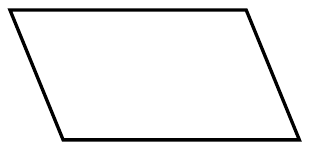
\includegraphics[width=2.4cm]{../gambar/simbol-2.png} & \textbf{\textit{Symbol Input/Output}} (simbol yang menunjukkan proses input atau output) \\
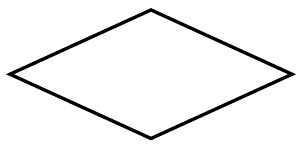
\includegraphics[width=2.4cm]{../gambar/simbol-3.png} & \textbf{\textit{Symbol Decision}} (simbol untuk kondisi yang akan menghasilkan beberapa kemungkinan jawaban/aksi) \\
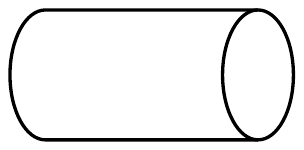
\includegraphics[width=2.4cm]{../gambar/simbol-4.png} & \textbf{\textit{Symbol Basisdata}} (simbol yang menunjukkan bahwa tempat penyimpanan data) \\
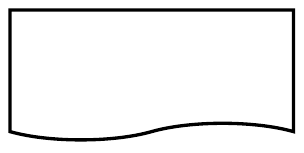
\includegraphics[width=2.4cm]{../gambar/simbol-5.png} & \textbf{\textit{Symbol Predefined Process}} (simbol untuk mempersiapkan penyimpanan yang akan digunakan sebagai tempat pengolahan di dalam \textit{storage}) \\
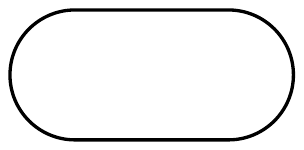
\includegraphics[width=2.4cm]{../gambar/simbol-6.png} & \textbf{\textit{Symbol Terminal}} (simbol untuk permulaan atau akhir dari suatu program) \\
\end{longtable}
\end{tanpagaris}

\subsection{Bab IV Hasil Penelitian dan Pembahasan}
Hasil Penelitian berisi data primer dan atau sekunder. Hasil penelitian yang bersifat kualitatif diungkapkan dalam bentuk narasi ilmiah sesuai dengan tujuan penelitian, sedangkan yang bersifat kuantitatif diungkapkan dalam bentuk tabel, grafik dan foto-foto. Data yang dikemukakan dalam bab hasil dan pembahasan, hendaknya bukan data murni, melainkan hasil olahan statistik, sedangkan data laboratorium atau lapangan yang diperoleh dapat dimasukkan dalam bentuk data murni di lampiran.

Penyajian hasil penelitian atau pengamatan dapat berupa teks, tabel, gambar, grafik dan foto. Hasil penelitian dapat memuat data utama, data penunjang, dan pelengkap yang diperlukan untuk memperkuat hasil penelitian menggunakan uji statistik, apabila dalam kondisi tertentu dimungkinkan tidak menggunakan uji statistik. Narasi hasil penelitian memuat ulasan makna yang terdapat dalam tabel, gambar, grafik dan foto; setiap tabel dan gambar harus dirujuk dan dijelaskan di dalam teks. Pada penelitian rekayasa, hasil dibagi menjadi hasil implementasi (wujud sistem, tampilan, rangkaian) dan hasil pengujian (data pengukuran sesuai indikator kinerja).

Pembahasan dikemukakan secara komprehensif terkait dengan hasil penelitian diperkuat dengan hasil-hasil peneliti lain atau \textit{textbook}. Ulasan dalam pembahasan dapat berupa penjelasan teoritis baik secara kualitatif dan kuantitatif: mengapa hasil demikian diperoleh, apa maknanya, bagaimana perbandingannya dengan penelitian terdahulu, dan apa keterbatasannya.

\subsection{Bab V Kesimpulan dan Saran}
\subsubsection{Kesimpulan}
Kesimpulan merupakan uraian singkat hasil penelitian dan pembahasan yang diperoleh (bukan kalimat statistik) dengan mengacu pada tujuan dan hipotesis penelitian yang dikaji. Kesimpulan ditulis berurutan sesuai rumusan masalah, singkat, tidak memuat sitasi, dan tidak memuat hal baru yang belum dibahas pada bab sebelumnya.

\subsubsection{Saran}
Saran merupakan uraian atau anjuran yang mengacu pada kesimpulan penelitian yang dapat dimanfaatkan oleh pihak yang berkepentingan, termasuk keterbatasan penelitian dan arah pengembangan penelitian selanjutnya.

\section{Bagian Akhir}

\subsection{Daftar Pustaka}
Daftar pustaka memuat sumber informasi ilmiah yang diacu untuk menyusun laporan penelitian, dan hanya memuat sumber yang benar-benar dikutip di dalam teks. Penulisan mengikuti gaya \textbf{APA edisi ke-7} (\textit{American Psychological Association}). Ketentuan umum:
\begin{enumerate}
\item kata DAFTAR PUSTAKA diketik dengan huruf kapital di bagian tengah atas halaman, tanpa nomor bab;
\item tiap pustaka diketik satu spasi, baris kedua dan seterusnya menjorok ke dalam 1,27 cm (\textit{hanging indent}), dan jarak antara pustaka yang satu dengan lainnya satu baris kosong;
\item pustaka disusun menurut abjad nama belakang penulis pertama (atau menurut judul bila tanpa penulis), \textbf{tanpa nomor urut};
\item pustaka dengan penulis pertama yang sama diurutkan dari tahun yang lebih lama; bila nama dan tahun sama, diberi huruf kecil di belakang tahun (2020a, 2020b);
\item nama penulis ditulis nama belakang diikuti inisial; untuk dua sampai 20 penulis, semuanya dicantumkan dan sebelum penulis terakhir diberi tanda \&;
\item judul artikel ditulis dengan huruf kapital hanya pada huruf pertama kalimat; judul buku, nama jurnal, dan nama prosiding dicetak miring;
\item sumber yang dapat berubah isinya (halaman web, laporan daring, video, repositori kode) diakhiri \textbf{tanggal akses} dengan bentuk \textit{Diakses pada tanggal bulan tahun, dari alamat URL};
\item artikel dengan DOI cukup mencantumkan DOI dalam bentuk URL tanpa tanggal akses.
\end{enumerate}

Pola penulisan berbagai jenis sumber beserta contoh lengkapnya terdapat pada Lampiran 6.

\subsection{Lampiran}
LAMPIRAN disajikan setelah daftar pustaka; kata LAMPIRAN dimuat di bagian atas tengah halaman, ditulis dengan huruf besar. Isi lampiran adalah hasil penelitian skripsi yang tidak dimasukkan ke dalam tubuh tulisan agar tidak mengganggu uraian, umumnya berupa tabel yang melebihi satu halaman, data mentah, peta lokasi penelitian, perhitungan statistik, program atau kode sumber, rangkaian dan skematik, serta prosedur pendukung penelitian. Tiap topik lampiran diberi nomor urut dengan judul yang jelas (LAMPIRAN 1, LAMPIRAN 2, dan seterusnya). Judul lampiran ditulis dengan huruf kecil, kecuali awal kalimat huruf kapital dan tanpa titik di akhir kalimat. Gambar dan tabel di dalam lampiran diberi awalan nomor lampiran, misalnya Gambar L2.1 dan Tabel L2.1.
